\section{Quiz Time}

\begin{frame}[plain,noframenumbering]
    \centering
    \scalebox{3}{Quiz Time}
\end{frame}

\begin{frame}{Quiz: Will it break ABI?}
    \textbf{Proposal:} make \texttt{std::vector<T>::push\_back} return a reference to the element in its new location

    \vspace*{5mm}

    \centering

    \scalebox{1.2}{\textcolor{vertexDarkRed}{\texttt{void}}\texttt{ push\_back(const T\&);}}

    \scalebox{2}{$\downarrow$}

    \scalebox{1.2}{\textcolor{vertexDarkRed}{\texttt{T\&}}\texttt{ push\_back(const T\&);}}
\end{frame}

\begin{frame}[fragile]{Quiz: Will it break ABI?}
    \begin{columns}[t]
        \begin{column}{.4\textwidth}
            \inputcpplisting{snippet7}
        \end{column}
        \begin{column}{.5\textwidth}
            \inputasmlisting{snippet7}
        \end{column}
    \end{columns}
\end{frame}

\begin{frame}[fragile]{Quiz: Will it break ABI?}
    Both, \texttt{void push\_back} and \texttt{T\& push\_back} have the same mangled name (Itanium ABI)
    \begin{itemize}
        \item \textbf{Two} definitions in the old and the new TU
        \item ODR violation
        \item Linker will pick only \textbf{one} definition (by \textbf{overwriting} the other)
        \item \textcolor{vertexDarkRed}{ABI break:} reading return value from \texttt{eax} when there is none
    \end{itemize}
\end{frame}

\begin{frame}{Quiz: Will it break ABI?}
    \textbf{Proposal:} make \texttt{std::vector<T>::emplace\_back} return a reference to the element in its new location

    \vspace*{5mm}

    \centering

    \scalebox{1.2}{\texttt{template<class... Args> }\textcolor{vertexDarkRed}{\texttt{void}}\texttt{ emplace\_back(Args\&\&...);}}

    \scalebox{2}{$\downarrow$}

    \scalebox{1.2}{\texttt{template<class... Args> }\textcolor{vertexDarkRed}{\texttt{T\&}}\texttt{ emplace\_back(Args\&\&...);}}
\end{frame}

\begin{frame}[fragile]{Quiz: Will it break ABI?}
    \inputcpplisting{snippet8}
% REMOVE_FOR_PRINT {
    \only<2>{%
% REMOVE_FOR_PRINT }
    \textbf{Mangled names:} (Itanium ABI)
    \begin{enumerate}
        \item \texttt{\_ZN6vectorIiE14emplace\_back\_1\textcolor{vertexDarkRed}{IJiEEEvDpOT\_}}
        \item \texttt{\_ZN6vectorIiE14emplace\_back\_2\textcolor{vertexDarkRed}{IJiEEERiDpOT\_}}
    \end{enumerate}
% REMOVE_FOR_PRINT {
    }
% REMOVE_FOR_PRINT }
\end{frame}

\begin{frame}[fragile]{Quiz: Will it break ABI?}
    \texttt{void emplace\_back} and \texttt{T\& emplace\_back} have different mangled names (\textit{cf.} \href{https://itanium-cxx-abi.github.io/cxx-abi/abi.html#mangle.function-type}{Itanium ABI: \textit{5.1.5.3 Function types}})
    \begin{itemize}
        \item Two definitions in the old and the new TU
        \item but no ODR violation
        \item \textcolor{vertexDarkRed}{No ABI break:} old code calls the old one, new code calls the new one ($\rightarrow$ proposal was accepted for \texttt{C++20}\,!)
    \end{itemize}
\end{frame}

\begin{frame}{Quiz: Will it break ABI?}
    \textbf{Proposal:} extend \texttt{std::lock\_guard<T>} to allow for a variadic set of heterogeneous mutexes

    \vspace*{5mm}

    \centering

    \scalebox{1.2}{\texttt{template<}\textcolor{vertexDarkRed}{\texttt{class Mutex}}\texttt{> class lock\_guard;}}

    \scalebox{2}{$\downarrow$}

    \scalebox{1.2}{\texttt{template<}\textcolor{vertexDarkRed}{\texttt{class... Mutexes}}\texttt{> class lock\_guard;}}
\end{frame}

\begin{frame}[fragile]{Quiz: Will it break ABI?}
    \begin{columns}[t]
        \begin{column}{.4\textwidth}
            \inputcpplisting{snippet9}
        \end{column}
        \begin{column}{.5\textwidth}
            \inputasmlisting{snippet9}
        \end{column}
    \end{columns}
\end{frame}

\begin{frame}[fragile]{Quiz: Will it break ABI?}
    \texttt{<class T> class} and \texttt{<class... T> class} have different mangled names (Itanium ABI)
    \begin{itemize}
        \item \textcolor{vertexDarkRed}{ABI break:} for example in \texttt{auto f(std::lock\_guard<M>\& lk);}
        \begin{itemize}
            \item \textit{cf.} \href{https://godbolt.org/z/Pex6Gx}{\texttt{godbolt.org/z/Pex6Gx}}
        \end{itemize}
        \item User compiles \texttt{f} using old \texttt{lock\_guard}
        \item User then tries to call it from a TU using new \texttt{lock\_guard}
        \item Mangled names don't match: linker error!
    \end{itemize}
\end{frame}

\begin{frame}{Quiz: Will it break ABI?}
    \textbf{Proposal:} change hashing by \texttt{std::hash} to improve performance of \texttt{std::unordered\_map} by 3-4x (\textit{cf.} \texttt{absl::node\_hash\_map})

    \vspace*{5mm}

% REMOVE_FOR_PRINT {
    \only<2>{%
% REMOVE_FOR_PRINT }
    \textcolor{vertexDarkRed}{\textbf{ABI break:}}
    \begin{itemize}
        \item Hash value for an object is computed in old TU and stored in map
        \item (Different) hash value is computed in new TU and used to lookup value in map
        \item \textbf{Semantic meaning of binary representation has changed!}
    \end{itemize}
% REMOVE_FOR_PRINT {
    }
% REMOVE_FOR_PRINT }
\end{frame}

\begin{frame}{Other Examples}
    More examples:
    \begin{itemize}
        \item \texttt{std::regex} currently is 10-100x slower than equivalents in Rust or Go (\textit{cf.} any talk of \href{https://youtu.be/8dKWdJzPwHw}{Hana Dusíková})
        \item Make \texttt{std::unique\_ptr} zero-overhead (\textit{cf.} Chandler Carruth, \href{https://youtu.be/rHIkrotSwcc}{\textit{There Are No Zero-cost Abstractions}})
        \item Add \texttt{std::int128\_t} which already is supported on more and more platforms
        \item Make \texttt{std::bitset} trivially destructible
        \item Exceptions (would be an entire talk on its own)
        \item \ldots 
    \end{itemize}

    \centering
    \scalebox{1.2}{(read \href{http://www.open-std.org/jtc1/sc22/wg21/docs/papers/2020/p2028r0.pdf}{\texttt{P2028}} and \href{http://www.open-std.org/jtc1/sc22/wg21/docs/papers/2020/p1863r1.pdf}{\texttt{P1863}} by Titus Winters for more information)}
\end{frame}

\section{Future Prospects}

\begin{frame}[plain,noframenumbering]
    \centering
    \scalebox{3}{Future Prospects}
\end{frame}

\begin{frame}{Future Prospects}
    \textbf{Break ABI with future releases:} move run-time failures to compile-time (when possible) by changing mangled name

    \begin{itemize}
        \item new namespaces: \textit{e.g.}, \texttt{std2::} or \texttt{std::abi42::}
        \begin{itemize}
            \item developers now have to choose between \texttt{std::optional} and \texttt{std2::optional} or duplicate code with overloading
            \item when will \texttt{std3::} arrive?
        \end{itemize}
        \item change entire mangling scheme: \textit{e.g.}, \texttt{\_Z} $\mapsto$ \texttt{\_Y} on Itanium
        \begin{itemize}
            \item Compiler vendors could ship both forms
        \end{itemize}
        \item Introduce version number (ABI break)
        \begin{itemize}
            \item MSVC does already include version numbers in DLLs (MSVCs users are used to recompile with each new version of Visual Studio \ldots)
        \end{itemize}
    \end{itemize}
\end{frame}

\begin{frame}{State-of-the-Art}
    \begin{itemize}
        \item No (major?) ABI breaks since \texttt{C++11} (\textbf{12 years in 2023!})
        \item \href{https://www.hyrumslaw.com/}{Hyrum's Law} (or \href{https://xkcd.com/1172/}{\texttt{xkcd.com/1172}}): passing ABI-unstable types across ABI boundaries happened to work for more than a decade. People rely on ABI stability, even though it was never explicitly promised.
        \item Expose C-APIs whenever possible
    \end{itemize}
\end{frame}

\begin{frame}{State-of-the-Art}
    \begin{columns}
        \begin{column}{.45\textwidth}
            \textbf{Standard Meeting, Prague 2020}
            \begin{itemize}
                \item \href{http://www.open-std.org/jtc1/sc22/wg21/}{WG21} is not in favor of an ABI break in \texttt{C++23} or \texttt{C++26}
                \item \href{http://www.open-std.org/jtc1/sc22/wg21/}{WG21} is in favor of an ABI break in a future version of C++
                \item \href{http://www.open-std.org/jtc1/sc22/wg21/}{WG21} will take time to consider proposals requiring an ABI break 
                \item \href{http://www.open-std.org/jtc1/sc22/wg21/}{WG21} will not promise stability forever
                \item \href{http://www.open-std.org/jtc1/sc22/wg21/}{WG21} wants to keep prioritizing performance over stability
            \end{itemize}
        \end{column}
        \begin{column}{.45\textwidth}
            \centering
            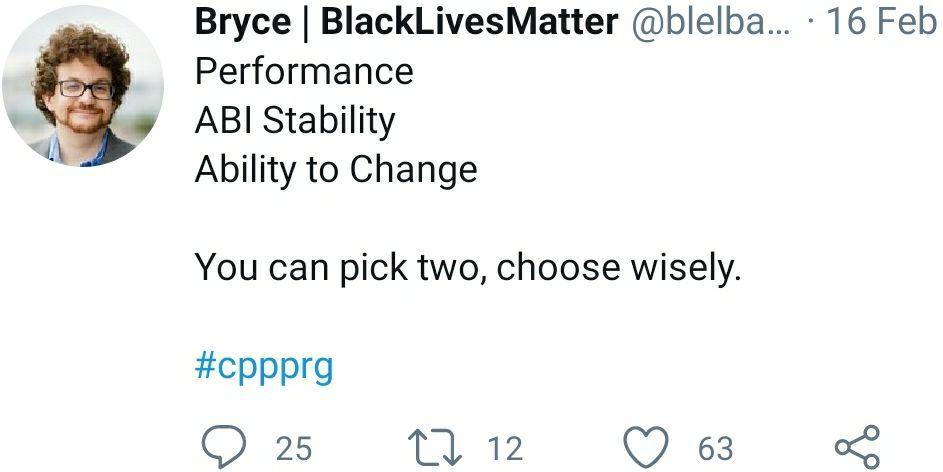
\includegraphics[width=\textwidth]{bryce_twitter.png}\\
            {\footnotesize \href{https://twitter.com/blelbach/status/1228962495865507840}{Twitter: \texttt{@blebach} (2020)}}

        \end{column}
    \end{columns}

    \vspace*{5mm}

    (\href{https://cor3ntin.github.io/posts/abi/}{Corentin Jabot: \textit{There was no applause. But I’m not sure we fully understood what we did and the consequences it could have.}})
\end{frame}

\begin{frame}{State-of-the-Art}
    \centering
    
\includegraphics[height=.8\textheight]{titus_twitter.png}\\
    {\footnotesize \href{https://twitter.com/TitusWinters/status/1224377740306132998}{Twitter: \texttt{@TitusWinters} (2020)}}
\end{frame}

\begin{frame}{Literature}
    \begin{itemize}
        \item \href{http://www.open-std.org/jtc1/sc22/wg21/docs/papers/2020/p2028r0.pdf}{Titus Winters, \texttt{P2028}: \textit{What is ABI, and What Should \href{http://www.open-std.org/jtc1/sc22/wg21/}{WG21} Do About It?}}
        \item \href{http://www.open-std.org/jtc1/sc22/wg21/docs/papers/2020/p1863r1.pdf}{Titus Winters, \texttt{P1863}: \textit{ABI - Now or Never}}
        \item \href{http://open-std.org/JTC1/SC22/WG21/docs/papers/2020/p1654r1.html}{Roger Orr, \texttt{P1654}: \textit{ABI breakage - summary of initial comments}}
        \item \href{https://cppcast.com/titus-winters-abi/}{Titus Winters on CppCast \#224: \textit{The C++ ABI}}
        \item \href{https://cppcast.com/john-lakos-large-scale-cpp/}{John Lakos on CppCast \#233: \textit{Large Scale C++}}
        \item \href{https://cor3ntin.github.io/posts/abi/}{Corentin Jabot on \texttt{cor3ntin.github.io/posts/abi/}: \textit{The Day The Standard Library Died}}
        \item \href{https://thephd.github.io/freestanding-noexcept-allocators-vector-memory-hole}{JeanHeyd Meneide on \texttt{thephd.github.io/freestanding-noexcept-allocators-vector-memory-hole}}
        \item \href{https://youtu.be/GRuX31P4Ric}{Danila Kutenin on \texttt{youtu.be/GRuX31P4Ric}: \textit{C++ STL best and worst performance features and how to learn from them}}
    \end{itemize}
\end{frame}
